\documentclass[11pt]{article}

\usepackage{graphicx}
\usepackage{wrapfig}
\usepackage{url}
\usepackage{wrapfig}
\usepackage{color}
\usepackage{marvosym}
\usepackage{enumerate}
\usepackage{tikz}
\usepackage{amsmath}
\usepackage{amssymb}
\usepackage{hyperref}
\usepackage{bbm}
\usepackage{verbatim}
\usepackage{bm}
\usepackage{caption}
\usepackage{subcaption}
\usepackage{tikz}
\usetikzlibrary{shapes, arrows, calc, positioning,matrix}
\tikzset{
data/.style={circle, draw, text centered, minimum height=3em ,minimum width = .5em, inner sep = 2pt},
empty/.style={circle, text centered, minimum height=3em ,minimum width = .5em, inner sep = 2pt},
}
\oddsidemargin 0mm
\evensidemargin 5mm
\topmargin -20mm
\textheight 240mm
\textwidth 160mm

\newcommand{\ztnodesize}{.6}

\DeclareMathOperator*{\argmin}{argmin}
\DeclareMathOperator*{\argmax}{argmax}

\newcommand{\vwi}{{\bf w}_i}
\newcommand{\vw}{{\bf w}}
\newcommand{\vx}{{\bf x}}
\newcommand{\vy}{{\bf y}}
\newcommand{\vxi}{{\bf x}_i}
\newcommand{\yi}{y_i}
\newcommand{\vxj}{{\bf x}_j}
\newcommand{\vxn}{{\bf x}_n}
\newcommand{\yj}{y_j}
\newcommand{\ai}{\alpha_i}
\newcommand{\aj}{\alpha_j}
\newcommand{\X}{{\bf X}}
\newcommand{\Y}{{\bf Y}}
\newcommand{\vz}{{\bf z}}
\newcommand{\msigma}{{\bf \Sigma}}
\newcommand{\vmu}{{\bf \mu}}
\newcommand{\vmuk}{{\bf \mu}_k}
\newcommand{\msigmak}{{\bf \Sigma}_k}
\newcommand{\vmuj}{{\bf \mu}_j}
\newcommand{\msigmaj}{{\bf \Sigma}_j}
\newcommand{\pij}{\pi_j}
\newcommand{\pik}{\pi_k}
\newcommand{\D}{\mathcal{D}}
\newcommand{\el}{\mathcal{L}}
\newcommand{\N}{\mathcal{N}}
\newcommand{\vxij}{{\bf x}_{ij}}
\newcommand{\vt}{{\bf t}}
\newcommand{\yh}{\hat{y}}
\newcommand{\code}[1]{{\footnotesize \tt #1}}
\newcommand{\alphai}{\alpha_i}

\renewcommand{\hat}[1]{\widehat{#1}}

\newcommand{\xij}{{x_{ij}}}
\DeclareMathAlphabet{\mathpzc}{OT1}{pzc}{m}{it}


\newcommand{\TODO}[1]{\textbf{\color{red}TODO: #1}}
\newcommand{\answer}[1]{\textbf{\color{red}Answer: #1}}



%%%%%%%%%%%%%%%%%%%%%%%%%%%%%%%%%%%%%%%%%%%%%%%%%%%%%%%%%%%%%%%%%%%%%%%%%%%%%%%%
% Gradescope-friendly boxes

\usepackage{tikz}
\usepackage[many]{tcolorbox}
\usepackage{float}
\usepackage{trimclip}
\usepackage{listings}
\usepackage{environ}% http://ctan.org/pkg/environ
\usepackage{wasysym}
\usepackage{array}



\bgroup
\def\arraystretch{1.5}
\newcolumntype{x}[1]{>{\centering\arraybackslash\hspace{0pt}}p{#1}}
\newcolumntype{z}[1]{>{\centering\arraybackslash}m{#1}}

%Arguments are 1 - height, 2 - box title
\newtcolorbox{textanswerbox}[2]{%
 width=\textwidth,colback=white,colframe=blue!30!black,floatplacement=H,height=#1,title=#2,clip lower=true,before upper={\parindent0em}}

 \newtcolorbox{eqanswerbox}[1]{%
 width=#1,colback=white,colframe=black,floatplacement=H,height=3em,sharp corners=all,clip lower=true,before upper={\parindent0em}}

 %Arguments are 1 - height, 2 - box title
 \NewEnviron{answertext}[2]{
        \noindent
        \marginbox*{0pt 10pt}{
        \clipbox{0pt 0pt 0pt 0pt}{
        \begin{textanswerbox}{#1}{#2}
        \BODY
        \end{textanswerbox}
        }
        }
}

%Arguments are 1 - height, 2 - box title, 3 - column definition
 \NewEnviron{answertable}[3]{
        \noindent
        \marginbox*{0pt 10pt}{
        \clipbox{0pt 0pt 0pt 0pt}{
        \begin{textanswerbox}{#1}{#2}
                \vspace{-0.5cm}
                        \begin{table}[H]
                        \centering
                        \begin{tabular}{#3}
                        \BODY
                        \end{tabular}
                        \end{table}
        \end{textanswerbox}
        }
        }
}

 %Arguments are 1 - height, 2 - box title, 3 - title, 4- equation label, 5 - equation box width
 \NewEnviron{answerequation}[5]{
        \noindent
        \marginbox*{0pt 10pt}{
        \clipbox{0pt 0pt 0pt 0pt}{
        \begin{textanswerbox}{#1}{#2}
                \vspace{-0.5cm}
                        \begin{table}[H]
                        \centering
                \renewcommand{\arraystretch}{0.5}% Tighter

                        \begin{tabular}{#3}
                                #4 =    &
                        \clipbox{0pt 0pt 0pt 0pt}{

                        \begin{eqanswerbox}{#5}
                        $\BODY$
                        \end{eqanswerbox}
                        } \\
                        \end{tabular}
                        \end{table}

        \end{textanswerbox}
        }
        }
}

 %Arguments are 1 - height, 2 - box title
 \NewEnviron{answerderivation}[2]{
        \noindent
        \marginbox*{0pt 10pt}{
        \clipbox{0pt 0pt 0pt 0pt}{
        \begin{textanswerbox}{#1}{#2}
       \BODY
        \end{textanswerbox}
        }
        }
}

\newcommand{\Checked}{{\LARGE \XBox}}%
\newcommand{\Unchecked}{{\LARGE \Square}}%
\newcommand{\TextRequired}{{\textbf{Place Answer Here}}}%
\newcommand{\EquationRequired}{\textbf{Type Equation Here}}%


\newcommand{\answertextheight}{5cm}
\newcommand{\answertableheight}{4cm}
\newcommand{\answerequationheight}{2.5cm}
\newcommand{\answerderivationheight}{14cm}

\newcounter{QuestionCounter}
\newcounter{SubQuestionCounter}[QuestionCounter]
\setcounter{SubQuestionCounter}{1}

\newcommand{\subquestiontitle}{Question \theQuestionCounter.\theSubQuestionCounter~}
\newcommand{\newquestion}{\stepcounter{QuestionCounter}\setcounter{SubQuestionCounter}{1}\newpage}
\newcommand{\newsubquestion}{\stepcounter{SubQuestionCounter}}



\pagestyle{myheadings}
\markboth{Homework 4}{Fall 2019 CS 475 Machine Learning: Homework 4}


\title{CS 475 Machine Learning: Homework 4\\EM and Graphical Models\\
\Large{Due: Wednesday November 20, 2019, 11:59pm}\\
100 Points Total \hspace{1cm} Version 1.5}
\author{}
\date{}

\begin{document}
\large
\maketitle
\thispagestyle{headings}

\vspace{-.5in}

{\bf Make sure to read from start to finish before beginning the assignment.}

\section{Programming (50 points)}


You will implement a Markov Random Field (MRF) for image segmentation. Please see section 19.4.3 of Kevin Murphy's textbook for a description of the model.
We will be providing a Python model framework/skeleton as before. Remember: \textbf{do not change the names of any of the files or command-line arguments.}

\subsection{Image Segmentation using MRFs}
The goal of image segmentation is to segment the objects displayed in an image into $K$ different groups.
Given a grayscale image containing $S$ pixels, the goal is to assign each pixel into one of these $K$ groups.
For example, for an image of an animal standing in a field, a 3 group segmentation may correspond to the animal, the sky and the ground. An example of such a segmentation can be seen in figure \ref{fig:segmentation}.

\begin{figure}\centering
    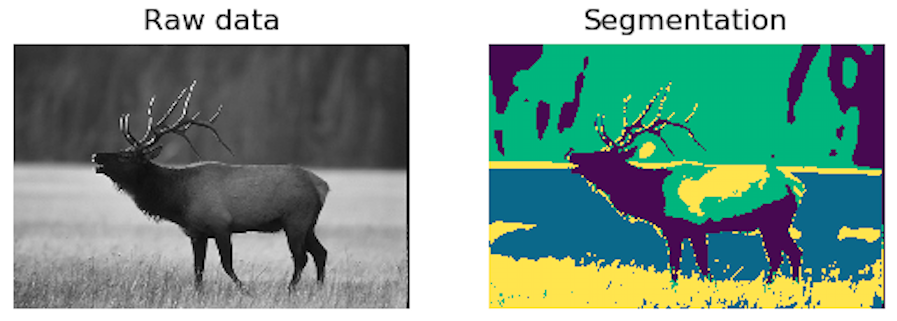
\includegraphics[width=90mm]{segmentation.png}
    \caption{An example of an image segmentation on a grayscale image.}
    \label{fig:segmentation}
\end{figure}


Segmentation models determine segments based on pixel color/values, where a segment contains pixel that all appear similarly. In this sense, segmentation is similar to pixel clustering. However, an image segmentation model also considers the position of pixels. Adjacent pixels are likely to belong to the same cluster.

In this assignment, you will implement and train an MRF that will assign each of the $S$ pixels in an image into one of $K$ discrete states. The MRF will encourages pixels to be assigned to segments with a similar color and many adjacent pixels. We will use the Berkeley Segmentation Dataset and Benchmark: \url{https://www2.eecs.berkeley.edu/Research/Projects/CS/vision/bsds/}



\subsection{MRF specification}
You will implement the Potts model, a type of MRF shown in Figure \ref{fig:potts-model} with the goal of clustering pixels in an image. From this perspective, each image is a dataset containing many pixels that will be clustered. As the distribution of pixel intensities will vary from image to image, the clustering results will look different in different images. Therefore, unlike models where parameters are trained over many images, parameters in the Potts model will be trained separately for each image. In this model, each pixel $s$ in the image corresponds to two random variables in the graphical model: $y_s$ and $x_s$.

\begin{figure}\centering
    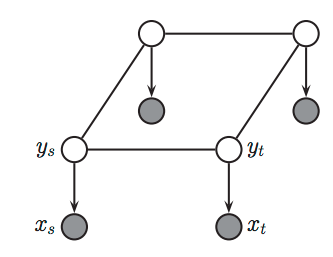
\includegraphics[width=90mm]{potts_model}
    \caption{Illustration of Potts model (image credit to Kevin Murphy's
      book).}
    \label{fig:potts-model}
\end{figure}

\begin{enumerate}
  \item $y_s \in {1, 2, ..., K}$ is a latent random variable for pixel $s$ that has $K$ possible states, where the value of $y_s$ indicates the segment.
  \item $x_s \in {0, ..., 255}$ is the observed intensity of pixel $s$.
\end{enumerate}

For notation, let $y=\{ (y_s) \}^S_{s=1}$ and $x=\{ (x_s) \}^S_{s=1}$.

\paragraph{Network structure:}
The Potts model connects each latent variable $y_s$ to the latent variables corresponding to neighboring (adjacent) pixels. Assuming pixel $s$ corresponds to the pixel in row $i$ and column $j$ of the image, the Potts model connects $y_s$ to four other pixels:
\begin{enumerate}
    \item The pixel in row $i+1$ and column $j$.
    \item The pixel in row $i-1$ and column $j$.
    \item The pixel in row $i$ and column $j+1$.
    \item The pixel in row $i$ and column $j-1$.
\end{enumerate}

A pixel on the boarder of the image will have fewer connections, e.g. a pixel in the corner will only have two adjacent pixels. Let $\mathpzc{N}(s)$ correspond to the neighbors of $s$.

\paragraph{Data likelihood:}
The joint likelihood of the full Potts model is:

\begin{equation}\label{eq:joint_likelihood}
  p(y, x \mid \theta, J) = p(y \mid J)\prod_{s=1}^S p(x_s \mid y_s,\theta) \end{equation}
  \\
  where $p(y \mid J)$ is the prior distribution on the latent variables, $y$. This prior distribution is parameterized by $J$, a model hyper-parameter that controls the strength of the connection between two adjacent pixels.
    $p(x_s \mid y_s, \theta)$ is the emission probability for pixel $s$, i.e. the likelihood of a pixel, $s$, observing the value $x_s$ given that it belongs state $y_s$. $\theta$ parameterizes emission probability distributions. Letting $s\sim t$ represent the set of pairs of pixels that share an edge in the MRF. We can expand equation \ref{eq:joint_likelihood} as follows:

\begin{equation}\label{eq:expanded_joint_likelihood}
  p(y, x \mid \theta, J)  = \left(\frac{1}{Z(J)}\prod_{s\sim t}\psi(y_s,y_t \mid J) \right)\prod_{s=1}^S p(x_s \mid y_s,\theta) \end{equation}
\begin{equation}\label{eq:partition_function}
  Z(J) = \sum_y \prod_{s\sim t}\psi(y_s,y_t \mid J)  \end{equation}
\\
where $\psi(y_s, y_t \mid J)$ is the edge potential, according to the MRF, between the segmentation for pixel $s$ and pixel $t$, and $Z(J)$ is the partition function.
\paragraph{Edge potentials:}
You will use the following potential function to model the interaction between two neighboring pixels:
\begin{equation}\label{eq:potential_function}
\psi(y_s, y_t \mid J)= \begin{cases}
      e^{J} & \text{if } y_s = y_t \\
      1 &  \text{otherwise}
   \end{cases}
\end{equation}

\paragraph{Emission probabilities:}

You will use a Gaussian likelihood to model the emission probability $p(x_s|y_s,\theta)$. Specifically when $y_s == k$:
\begin{equation}\label{eq:emission_function}
p(x_s|y_s=k,\theta)= \mathcal{N}(x_s | \mu_k, \sigma_k)
\end{equation}
\\
where $\mu_k$ and $\sigma_k$ are the mean and standard deviation parameters, respectively, defining the univariate Gaussian distribution corresponding to state $k$. The parameter $\theta$ corresponds to $\{ (\mu_k, \sigma_k) \}^K_{k=1}$.



\subsection{MRF Parameter Learning}

Learning the parameters of the Potts model corresponds to:

\begin{enumerate}
    \item Computing the expected value of the posterior distribution on the latent variables: $p(y|x,\theta,J)$
    \item Optimizing the parameters $\theta$ defining the emission probabilities $p(x_s|y_s, \theta)$.
\end{enumerate}

Since this is likelihood maximization with latent variables we will use EM.

\paragraph{E-step: Variational Inference:}
In each iteration of EM, the E-step computes estimates of $p(y|x,\theta,J)$, where $\theta$ is fixed at its optimal value according to the most recent M-step. As $\{ (x_s) \}^S_{s=1}$ is observed, $p(y|x,\theta,J) \propto p(y,x|\theta,J)$. Therefore, the E-step involves computing the distribution specified in equation \ref{eq:expanded_joint_likelihood}. Unfortunately however, the partition function $Z(J)$ becomes intractable to compute when there are more than a few pixels. Notice that the graph is not tree-structured, so we cannot rely on the exact inference algorithms we learned in class.

Instead, we approximate the posterior $p(y|x,\theta,J)$ using Mean Field Variational Inference (See {\scriptsize \url{https://www.cs.cmu.edu/~epxing/Class/10708-17/notes-17/10708-scribe-lecture13.pdf}} for an overview of Variational Inference).

Mean Field Variational Inference approximates the complex posterior distribution $p(y|x,\theta,J)$ with a fully factorized distribution $q(y)$:
\begin{equation}\label{eq:vi_1}
    p(y|x,\theta,J) \approx q(y) = \prod_{s=1}^S q(y_s,p_s)
\end{equation}
\\
where $p_s\in \mathbb{R}^K$ parameterizes the variational distribution $q_s$ to model the (categorical) posterior probability that $y_s$ is equal to each of the K states. Specifically:
\begin{equation}
    q(y_s=k,p_s)=p_s^{(k)}
\end{equation}
\begin{equation}
    \sum_{k=1}^K p_s^{(k)} =1
\end{equation}\\
 A schematic of the factorization of the MRF posterior according to Mean Field can be found in figure \ref{fig:mean-field}. This is a gross simplification of the true distribution, but the simplification makes inference much easier. We fit this simplified distribution to match, as closely as possible, the true distribution.

\begin{figure}\centering
    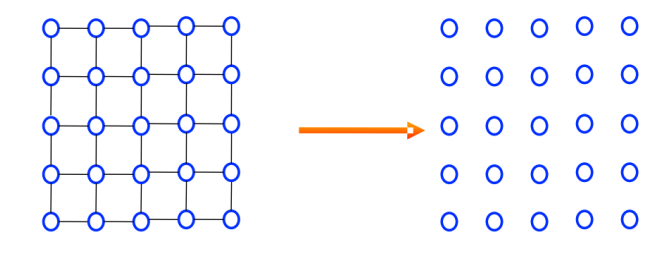
\includegraphics[width=90mm]{mean_field.png}
    \caption{Illustration of Mean Field Variational Approximation (image credit to Kevin Murphy's
      book).}
    \label{fig:mean-field}
\end{figure}

\paragraph{Variational Inference Pseudocode}

We provide the following pseudocode to optimize the Variational parameters ($p_s$) to make the Variational distributions ($q_s$) as similar as possible to the true posterior $p(y|x,\theta,J)$ in terms of KL-Divergence, a metric to measure the difference between two probability distributions.
\begin{enumerate}
    \item Initialize the Variational parameters $\{ (p_s) \in \mathbb{R}^K \}^S_{s=1}$ at random while ensuring $\sum_{k=1}^K p_s^{(k)} = 1$. Note: This step is already implemented in the Python skeleton (see function \textit{initialize\_variational\_parameters()} in \textit{models.py}) to ensure consistency between students.
    \item For iteration $m = 1$ to $M$:
    \begin{enumerate}[(a)]
        \item For pixel $s = 1$ to $S$:
            \begin{enumerate}[(i)]
                \item For each state $k$, update $p_s^{(k)}$ while fixing variational approximations of all other pixels to their most recent updated value according to:
                \begin{equation}\label{eq:vi_update}
                q(y_s=k,p_s)=\frac{\mathcal{N}(x_s \mid \mu_k, \sigma_k) \exp(\sum_{i\in \mathpzc{N}(s)}J\: q(y_i=k,p_i))}{\sum_{k'=1}^K \mathcal{N}(x_s \mid \mu_{k'}, \sigma_{k'}) \exp(\sum_{i\in \mathpzc{N}(s)}J\: q(y_i=k',p_i)) }
                \end{equation}

            \end{enumerate}
    \end{enumerate}
\end{enumerate}

$M$ is hyperparameter controlling the number of Variational inference iterations to run.\\\\
To ensure consistency between students: when looping through pixels please use an outer loop to iterate across rows of the image and an inner loop to iterate across columns of the image.

\paragraph{M-step: Maximum Likelihood Estimation:}
The M-step will update the parameters of the Potts model $\theta=\{ (\mu_k, \sigma_k) \}^K_{k=1}$ given the most recent E-step's variational approximations to the posterior ($q(y_s,p_s)$).\\\\
The updates are as follows. For state $k = 1$ to $K$:
\begin{itemize}
\item $\hat{\mu_k}=\frac{\sum_{s=1}^S q(y_s=k,p_s)x_s}{\sum_{s=1}^S q(y_s=k,p_s)}$
\item $\hat{\sigma^2_k}=\frac{\sum_{s=1}^S q(y_s=k,p_s)(x_s -\hat{\mu_k})^2}{\sum_{s=1}^S q(y_s=k,p_s)}$
\end{itemize}

\paragraph{Expectation-Maximization Pseudocode:}
We now summarize the entire EM procedure.
\begin{enumerate}
\item Initialize $\theta^{(0)}=\{ (\mu_k, \sigma_k) \}^K_{k=1}$ at random. Specifically, randomly assign $\mu_k \: \forall k$ to integers between $10$ and $240$ (inclusive) and set $\sigma_k=10 \:\forall k$. This step is already implemented in the Python skeleton (see function \textit{initialize\_theta\_parameters()} in \textit{models.py}) to ensure consistency between students.
\item For iteration $n = 1$ to $N$:
    \begin{enumerate}[(a)]
        \item E-Step: Run Variational Inference to generate $q(y_s,p_s)^{(n)} \: \forall s$ while keeping $\theta$ fixed at $\theta^{(n-1)}$
        \item M-Step: Use Maximum Likelihood to learn $\theta^{(n)}$ while keeping $q(y_s,p_s)$ fixed at $q(y_s,p_s)^{(n)}$
    \end{enumerate}
\item Run E-step one more time to generate $q(y_s,p_s)^{(N+1)} \: \forall s$ while keeping $\theta$ fixed at $\theta^{(N)}$.
\item For pixel $s = 1$ to $S$:
    \begin{enumerate}[(a)]
        \item Compute most likely state of pixel $s$ according to $q(y_s,p_s)^{(N+1)}$. States should be encoded $\{0,..,K-1\}$. If there is a tie (ie. two states have equal probability), select the state corresponding to the lower number.
    \end{enumerate}


\end{enumerate}

$N$ is hyperparameter controlling the number of EM iterations to run.

\subsection{Implementation Details}
Your code must correctly implement the behavior described by the following command line options, which are passed in as arguments to the constructor of your implementation
in models.py.
\begin{itemize}
    \item {\tt--edge-weight} Model hyper-parameter controlling the MRF prior distribution ($J$).
    \item {\tt --num-states} Model hyper-parameter controlling the number of MRF latent states ($K$).
    \item {\tt --n-em-iterations} Model hyper-parameter controlling the number of EM iterations ($N$).
    \item {\tt --random-seed} Integer specifying random seed to be used to ensure consistency of results between students.
    \item {\tt --n-vi-iterations} Model hyper-parameter controlling the number of iterations to use during Variational Inference ($M$).
    \item {\tt --train-data} A string corresponding to the name and location of the image file.
    \item {\tt --model-file} A string corresponding to where to store the model parameters
    \item {\tt --predictions-file} A string corresponding to where to store model predictions. \textit{main.py} will generate a tab-separated matrix to save here, where the matrix is the shape as the input image (from --train-data). Each row of the matrix  corresponds to a row of the input image (in pixel space) and each column corresponds to a column of the input image. Each element of this matrix corresponds to the most likely state of the corresponding pixel according to the fitted MRF. States should be encoded $\{0,..,K-1\}$.
    \item {\tt --visualize-predictions-file} A string corresponding to where to store a plot that jointly shows the raw image as well as image with pixels colored according to your segmentation.
\end{itemize}




\subsection{Examples}
We have provided four images for you to train your model and evaluate your clustering: \textit{image\_1.jpg}, \textit{image\_2.jpg}, \textit{image\_3.jpg}, \textit{image\_4.jpg}. \\\\
As an example of how the code should be run: the following trains an MRF on a training image image\_1.jpg:
\begin{footnotesize}
\begin{verbatim}
python3 main.py --train-data image_1.jpg --model-file train.model \
     --predictions-file train.predictions --algorithm mrf --edge-weight 1.2 --num-states 3 \
     --visualize-predictions-file segmentation_view.png
\end{verbatim}
\end{footnotesize}

\subsection{Evaluating segmentations}

We provide a script called \textit{compute\_accuracy.py} which will compute the accuracy of your state predictions relative to correct segmentations that we provide. We provide two correct segmentations for you to compare your results to:
\begin{enumerate}
    \item {\tt image\_1.true\_predictions}: A predictions file for \textit{image\_1.jpg} generated using the following parameters:\begin{verbatim} --edge-weight 1.2 --num-states 4 --random-seed 1 \ 
    --n-em-iterations 3 --n-vi-iterations 3
    \end{verbatim}
    \item {\tt image\_2.true\_predictions}: A predictions file for \textit{image\_2.jpg} generated using the following parameters:\begin{verbatim} --edge-weight 1.2 --num-states 4 --random-seed 1 \ 
    --n-em-iterations 3 --n-vi-iterations 3
    \end{verbatim}
\end{enumerate}

Note: your state predictions will only be comparible with the correct segmentations if you train your model using the above parameter settings. This script can be run using the following command:\\
\begin{footnotesize}
\begin{verbatim}
python3 compute_accuracy.py image_1.true_predictions image_1.predictions
\end{verbatim}
\end{footnotesize}

Where \textit{image\_1.true\_predictions} is the provided correct segmentation and \textit{image\_1.predictions} is your state predictions file.

\newpage
\section{Analytical (50 points)}


\subsection{D-separation in Graphical Models (20 points)}

\subsubsection{Directed (8 points)}
Consider the directed graphical model below. For each question, decide whether the sets
\textbf{A} and \textbf{B} are d-separated given set \textbf{C}.  Change \verb|\Unchecked| to \verb|\Checked| to provide your answer.
Additionally, explain your answer in terms of the rules of d-separation. 

\vspace{10pt}
\begin{center}
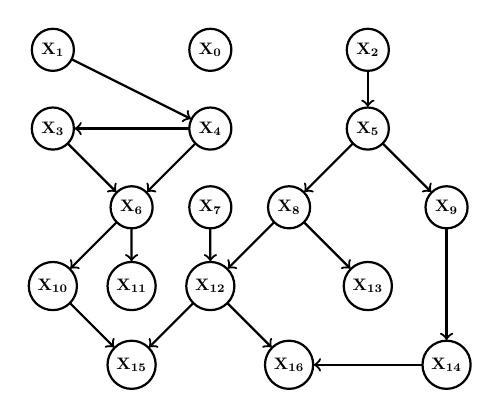
\begin{tikzpicture}[style=thick,scale=1]
\begin{scope}[shape=circle,minimum size=0.1cm]
\tikzstyle{every node}=[draw,fill]
\node[fill=none,scale=\ztnodesize] (X_0) at (2,4) {$\mathbf{X_0}$};
\node[fill=none,scale=\ztnodesize] (X_1) at (0,4) {$\mathbf{X_1}$};
\node[fill=none,scale=\ztnodesize] (X_2) at (4,4) {$\mathbf{X_2}$};
\node[fill=none,scale=\ztnodesize] (X_3) at (0,3) {$\mathbf{X_3}$};
\node[fill=none,scale=\ztnodesize] (X_4) at (2,3) {$\mathbf{X_4}$};
\node[fill=none,scale=\ztnodesize] (X_5) at (4,3) {$\mathbf{X_5}$};
\node[fill=none,scale=\ztnodesize] (X_6) at (1,2) {$\mathbf{X_6}$};
\node[fill=none,scale=\ztnodesize] (X_7) at (2,2) {$\mathbf{X_7}$};
\node[fill=none,scale=\ztnodesize] (X_8) at (3,2) {$\mathbf{X_8}$};
\node[fill=none,scale=\ztnodesize] (X_9) at (5,2) {$\mathbf{X_9}$};
\node[fill=none,scale=\ztnodesize] (X_10) at (0,1) {$\mathbf{X_{10}}$};
\node[fill=none,scale=\ztnodesize] (X_11) at (1,1) {$\mathbf{X_{11}}$};
\node[fill=none,scale=\ztnodesize] (X_12) at (2,1) {$\mathbf{X_{12}}$};
\node[fill=none,scale=\ztnodesize] (X_13) at (4,1) {$\mathbf{X_{13}}$};
\node[fill=none,scale=\ztnodesize] (X_14) at (5,0) {$\mathbf{X_{14}}$};
\node[fill=none,scale=\ztnodesize] (X_15) at (1,0) {$\mathbf{X_{15}}$};
\node[fill=none,scale=\ztnodesize] (X_16) at (3,0) {$\mathbf{X_{16}}$};
\draw [->] (X_1) -- (X_4);
\draw [->] (X_2) -- (X_5);
\draw [->] (X_4) -- (X_3);
\draw [->] (X_3) -- (X_6);
\draw [->] (X_4) -- (X_6);
\draw [->] (X_5) -- (X_9);
\draw [->] (X_5) -- (X_8);
\draw [->] (X_6) -- (X_10);
\draw [->] (X_6) -- (X_11);
\draw [->] (X_7) -- (X_12);
\draw [->] (X_8) -- (X_12);
\draw [->] (X_8) -- (X_13);
\draw [->] (X_9) -- (X_14);
\draw [->] (X_10) -- (X_15);
\draw [->] (X_12) -- (X_15);
\draw [->] (X_12) -- (X_16);
\draw [->] (X_14) -- (X_16);
\end{scope}
\end{tikzpicture}
\end{center}



\renewcommand{\answertextheight}{2.cm}

\begin{enumerate}[(a)]
\item {${\bf A} = \{x_1\}$, ${\bf B} = \{x_9\}$, ${\bf C} = \{x_8,x_{16}\}$}

\begin{answertext}{\answertextheight}{}
  \Unchecked Yes\\
  \Unchecked No

\end{answertext}

\item {${\bf A} = \{x_{11}\}$, ${\bf B} = \{x_{13}\}$, ${\bf C} = \{x_1,x_{15}\}$}

\begin{answertext}{\answertextheight}{}
  \Unchecked Yes\\
  \Unchecked No

\end{answertext}


\item ${\bf A} = \{x_4, x_0\}$, ${\bf B} = \{x_5, x_{13}\}$, ${\bf C} = \{x_{10},x_{16}\}$

\begin{answertext}{\answertextheight}{}
  \Unchecked Yes\\
  \Unchecked No

\end{answertext}


\item ${\bf A} = \{x_3, x_4\}$, ${\bf B} = \{x_{13},x_9\}$, ${\bf C} = \{x_7,x_{15},x_{16}\}$

\begin{answertext}{\answertextheight}{}
  \Unchecked Yes\\
  \Unchecked No

\end{answertext}


\end{enumerate}

\newpage
\subsubsection{Undirected (8 points)}
Suppose we take the same graph structure, but make the edges undirected.  This
change means that the directed version and undirected version will make
different conditional-independence assertions.  Again, for each of the following
questions, decide whether the sets \textbf{A} and \textbf{B} are d-separated
given set \textbf{C}. Additionally, explain your answer in terms of the rules of d-separation. 

\vspace{10pt}
\begin{center}
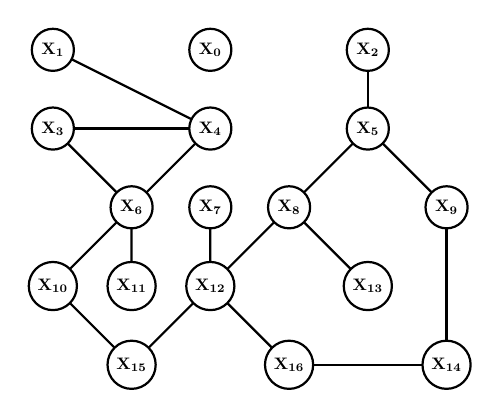
\begin{tikzpicture}[style=thick,scale=1]
\begin{scope}[shape=circle,minimum size=0.1cm]
\tikzstyle{every node}=[draw,fill]
\node[fill=none,scale=\ztnodesize] (X_0) at (2,4) {$\mathbf{X_0}$};
\node[fill=none,scale=\ztnodesize] (X_1) at (0,4) {$\mathbf{X_1}$};
\node[fill=none,scale=\ztnodesize] (X_2) at (4,4) {$\mathbf{X_2}$};
\node[fill=none,scale=\ztnodesize] (X_3) at (0,3) {$\mathbf{X_3}$};
\node[fill=none,scale=\ztnodesize] (X_4) at (2,3) {$\mathbf{X_4}$};
\node[fill=none,scale=\ztnodesize] (X_5) at (4,3) {$\mathbf{X_5}$};
\node[fill=none,scale=\ztnodesize] (X_6) at (1,2) {$\mathbf{X_6}$};
\node[fill=none,scale=\ztnodesize] (X_7) at (2,2) {$\mathbf{X_7}$};
\node[fill=none,scale=\ztnodesize] (X_8) at (3,2) {$\mathbf{X_8}$};
\node[fill=none,scale=\ztnodesize] (X_9) at (5,2) {$\mathbf{X_9}$};
\node[fill=none,scale=\ztnodesize] (X_10) at (0,1) {$\mathbf{X_{10}}$};
\node[fill=none,scale=\ztnodesize] (X_11) at (1,1) {$\mathbf{X_{11}}$};
\node[fill=none,scale=\ztnodesize] (X_12) at (2,1) {$\mathbf{X_{12}}$};
\node[fill=none,scale=\ztnodesize] (X_13) at (4,1) {$\mathbf{X_{13}}$};
\node[fill=none,scale=\ztnodesize] (X_14) at (5,0) {$\mathbf{X_{14}}$};
\node[fill=none,scale=\ztnodesize] (X_15) at (1,0) {$\mathbf{X_{15}}$};
\node[fill=none,scale=\ztnodesize] (X_16) at (3,0) {$\mathbf{X_{16}}$};
\draw [-] (X_1) -- (X_4);
\draw [-] (X_2) -- (X_5);
\draw [-] (X_4) -- (X_3);
\draw [-] (X_3) -- (X_6);
\draw [-] (X_4) -- (X_6);
\draw [-] (X_5) -- (X_9);
\draw [-] (X_5) -- (X_8);
\draw [-] (X_6) -- (X_10);
\draw [-] (X_6) -- (X_11);
\draw [-] (X_7) -- (X_12);
\draw [-] (X_8) -- (X_12);
\draw [-] (X_8) -- (X_13);
\draw [-] (X_9) -- (X_14);
\draw [-] (X_10) -- (X_15);
\draw [-] (X_12) -- (X_15);
\draw [-] (X_12) -- (X_16);
\draw [-] (X_14) -- (X_16);
\end{scope}
\end{tikzpicture}
\end{center}


\begin{enumerate}[(a)]
\item {${\bf A} = \{x_1\}$, ${\bf B} = \{x_9\}$, ${\bf C} = \{x_8,x_{16}\}$}

\begin{answertext}{\answertextheight}{}
  \Unchecked Yes\\
  \Unchecked No

\end{answertext}

\item {${\bf A} = \{x_{11}\}$, ${\bf B} = \{x_{13}\}$, ${\bf C} = \{x_1,x_{15}\}$}

\begin{answertext}{\answertextheight}{}
  \Unchecked Yes\\
  \Unchecked No

\end{answertext}


\item ${\bf A} = \{x_4, x_0\}$, ${\bf B} = \{x_5, x_{13}\}$, ${\bf C} = \{x_{10},x_{16}\}$

\begin{answertext}{\answertextheight}{}
  \Unchecked Yes\\
  \Unchecked No

\end{answertext}


\item ${\bf A} = \{x_3, x_4\}$, ${\bf B} = \{x_{13},x_9\}$, ${\bf C} = \{x_7,x_{15},x_{16}\}$

\begin{answertext}{\answertextheight}{}
  \Unchecked Yes\\
  \Unchecked No

\end{answertext}

\end{enumerate}



\subsubsection{More questions (4 points)}
Let $X = (X_1, . . . , X_{16})^T$ be a random vector with distribution given by the graphical model.  Consider variable $X_2$.

\renewcommand{\answertextheight}{8cm}

\begin{enumerate}[(a)]
\item What is the minimal subset of the variables, $A\subset \mathcal{X}
  -\{X_2\}$, such that $X_2$ is independent of the rest of the variables
  ($\mathcal{X} - (A\cup{\{ X_2\}}$)) given A? Justify your answer.

\begin{answertext}{\answertextheight}{}
\end{answertext}

\item Answer the same question for the undirected network.

\begin{answertext}{\answertextheight}{}
\end{answertext}

\end{enumerate}




\newpage
\subsection{EM and Naive Bayes (30 points)}

\paragraph{Background}
The Naive Bayes graphical model assumes that all features in a $m$-dimensional
$X \in \mathcal{X}^m$ are conditionally independent given the label $Y$.  Let
$\mathcal{Y}$ be the domain of the random variable $Y$.  A Naive Bayes
classifier can be represented as a graphical model,

\begin{center}
  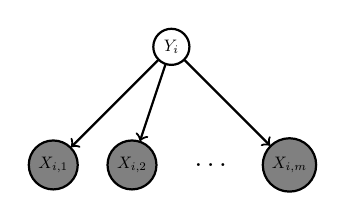
\begin{tikzpicture}[style=thick]
    \begin{scope}[shape=circle,minimum size=0.1cm]
      \tikzstyle{every node}=[draw,fill]
      \node[fill=none,scale=\ztnodesize] (root) at (2.5,1.5) {$Y_i$};
      \node[fill=gray,scale=\ztnodesize] (q_1) at (1,0) {$X_{i,1}$};
      \node[fill=gray,scale=\ztnodesize] (q_2) at (2,0) {$X_{i,2}$};
      \node[fill=none,draw=none] (q_3) at (3,0) {$\ldots$};
      \node[fill=gray,scale=\ztnodesize] (q_m) at (4,0) {$X_{i,m}$};
      \draw [->] (root) -- (q_1);
      \draw [->] (root) -- (q_2);
      \draw [->] (root) -- (q_m);
    \end{scope}
  \end{tikzpicture}
\end{center}


\noindent When $X$ and $Y$ are fully observed, the Naive Bayes model's likelihood
function is
\begin{equation}
  p( \{ \langle \langle x_{i,1}, \ldots, x_{i,m} \rangle, y_i \rangle \}_{i=1}^n )
  = \prod_{i=1}^n p(y_i) \prod_{j=1}^m p(x_{i,j} \mid y_i)\label{fully-observed}
\end{equation}

\noindent In terms of parameters, we write the likelihood as
$$
= \prod_{i=1}^n \theta_{y_i} \prod_{j=1}^m \theta_{x_{i,j} \mid y_i}
$$

\subsubsection{Parameters (4 points)}

\begin{enumerate}[(a)]

\item If our model has $m$ features with $n_X = |\mathcal{X}|$, and $n_Y =
|\mathcal{Y}|$ possible values for the label, how many parameters does the Naive
Bayes model have?  Give a big-$\mathcal{O}$ expression and briefly justify your
answer.

\begin{answertext}{2in}{}
\end{answertext}

\newpage
\item Not all settings to the parameter vector will give a valid interpretation
as a (prior or conditional) probability distribution.  Describe the necessary
constraints on our parameter vector $\theta$.  Be precise.

\begin{answertext}{2.5in}{}
  
\end{answertext}

\end{enumerate}


\subsubsection{Partially labeled training (26 points)}
Now we consider a \emph{semi-supervised} learning scheme with $n$ observations,
in which $X$ is observed for all training examples, but $Y$ is only
\emph{partially} observed: rather than observing the event $(Y = y_i)$, we
observe the event $(Y_i \in \mathcal{Y}_i)$ for some (nonempty) example-specific
subset $\mathcal{Y}_i \subseteq \mathcal{Y}$. Thus, our training data is a set
of pairs $\mathcal{D} = \{ \langle \langle x_{i,1}, \ldots, x_{i,m} \rangle,
\mathcal{Y}_i \rangle \}_{i=1}^n$.


\begin{enumerate}[(a)]
\item (6 points) \label{partial-likelihood} Because some of labels $Y_i$ are missing, the
  likelihood function in equation \ref{fully-observed} does not apply.  Write
  down the likelihood function for our partially labeled dataset.  You may use
  the $p()$ notation instead of $\theta$, if you prefer. [Hint: Check for
    yourself that when $\mathcal{Y}_i$ always has one element in it that you
    recover the fully observed case.]

\begin{answertext}{1.5in}{}
\end{answertext}

\newpage
\item (7 points) EM algorithm (E-step): The E-step for our model computes an approximate
  posterior distribution $q( Y_i = y \mid x_{i})$ over the missing labels using the current parameter
  estimate, $\widehat{\theta}$. [Hint: the posterior should put zero
    probability on the event that $(Y_i \notin \mathcal{Y}_i)$ and it should
    some to one over $y \in \mathcal{Y}$.]\looseness=-1

\vspace{10pt}
\noindent For $i \in \{1, \ldots, n\}$ and $y \in \mathcal{Y}$, the posterior is the
following distribution

\begin{answertext}{3in}{}
$q( Y_i = y \mid x_{i} ) = $\\
\end{answertext}

\item (7 points) EM algorithm (M-step): Write down the M-step objective function using the
  approximate posterior, $q$, that you defined in the previous question.  There is no need to solve
  the optimization problem, just write it down clearly.

\begin{answertext}{3in}{}
\end{answertext}

\newpage
\item (2 points) Could we optimize the data likelihood (your solution to part
  (\ref{partial-likelihood})) with a gradient-based optimization algorithm
  instead of EM?

\begin{answertext}{2in}{}
\end{answertext}

\item (4 points) What if we wanted to support real-valued features where
  $\mathcal{X} = \mathbb{R}$?  What would be a reasonable way to parameterize
  the label-conditioned feature distribution $p(x_j \mid y)$?  How many
  parameters does the new model have?\looseness=-1

\begin{answertext}{3in}{}
\end{answertext}

\end{enumerate}

\newpage
\section{What to Submit}
In this assignment you will submit two things.
\begin{enumerate}
\item \textbf{Submit your code (.py files) to cs475.org as a zip file}. \textbf{Your code must be uploaded as code.zip with your code in the root directory}. By `in the root directory,' we mean that the zip should contain \texttt{*.py} at the root (\texttt{./*.py}) and not in any sort of substructure (for example \texttt{hw1/*.py}). One simple way to achieve this is to zip using the command line, where you include files directly (e.g., \texttt{*.py}) rather than specifying a folder (e.g., \texttt{hw1}):
\begin{verbatim}
zip code.zip *.py
\end{verbatim}

A common mistake is to use a program that automatically places your code in a subfolder. It is your job to make sure you have zipped your code correctly.

We will run your code using the exact command lines described earlier, so make sure it works ahead of time, and make sure that it doesn't crash when you run it on the test data. A common mistake is to change the command line flags. If you do this, your code will not run.

Remember to submit all of the source code, including what we have provided to you. We will include {\tt requirements.txt} and provide the data, but nothing else.

\item \textbf{Submit your writeup to gradescope.com}. \textbf{Your writeup must be compiled from latex and uploaded as a PDF}. The writeup should contain all of the answers to the analytical questions asked in the assignment. Make sure to include your name in the writeup PDF and to use the provided latex template for your answers following the distributed template. You will submit this to the assignment called ``Homework 4: EM and Graphical Models: Written''.


\end{enumerate}


You will need to create an account on gradescope.com and signup for this class. The course is \href{https://gradescope.com/courses/21552}{\url{https://gradescope.com/courses/21552}}. Use entry code {\tt M6ZX2X}. See this video for instructions on how to upload a homework assignment: \href{https://www.youtube.com/watch?v=KMPoby5g_nE}{\url{https://www.youtube.com/watch?v=KMPoby5g_nE}}.

\section{Questions?}
Remember to submit questions about the assignment to the appropriate group on Piazza: \href{https://piazza.com/class/jkqbzabvyr15up}{\url{https://piazza.com/class/jkqbzabvyr15up}}.

\end{document}



